% erklaerung.tex
% Eigenständigkeitserklärung

\cleardoublepage

%\chapter{Erklärung}
%\label{chapter:erklaerung}

\newpage
%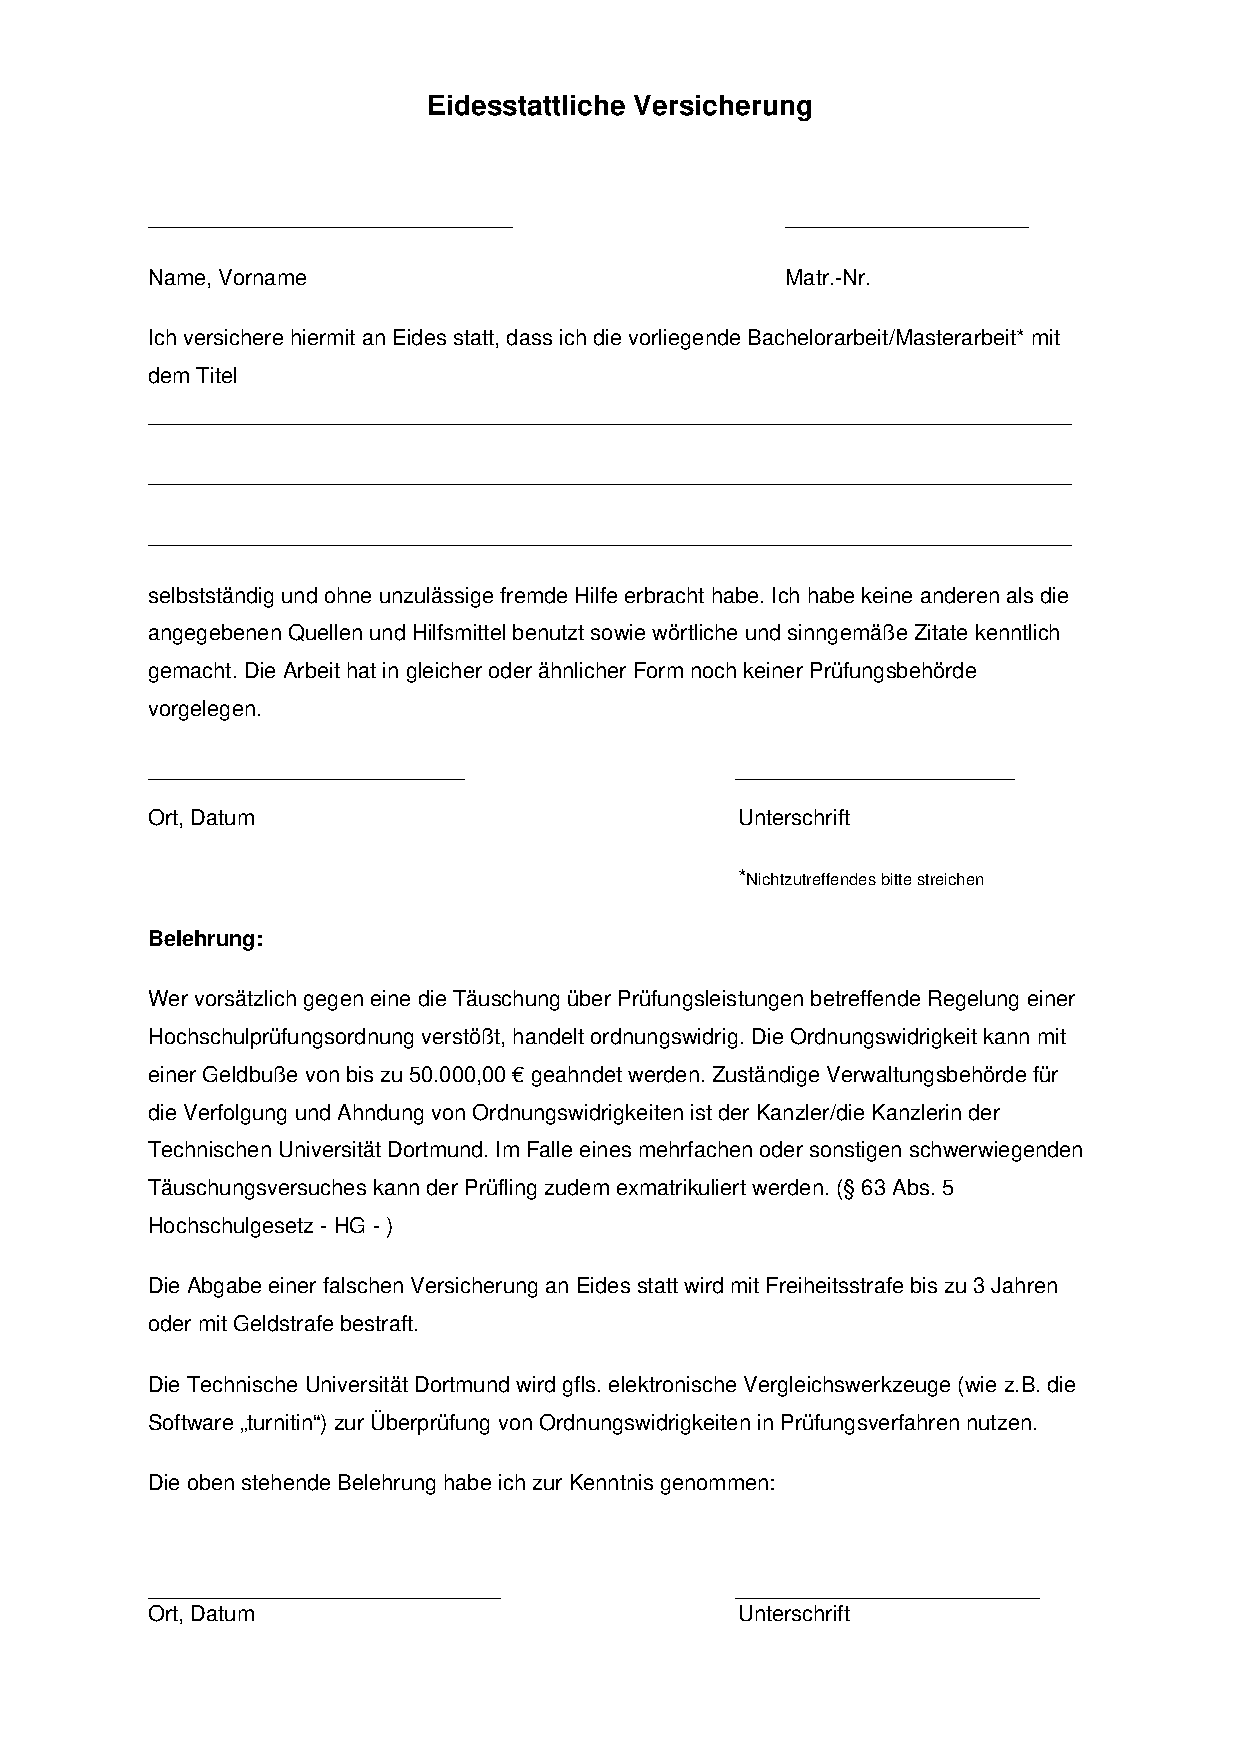
\includegraphics[scale=0.9]{bilder/eid.pdf}
\noindent\large{\textbf{Eidesstattliche Versicherung}}\newline

\noindent Hiermit versichere ich, Marcel Ebbrecht, Matrikel 111338, geboren am 09.11.1983 in Kassel, an Eides statt, dass ich die vorliegende Bachelorarbeit mit dem Titel \textbf{\glqq Energieeffizientes Routing in Ad-Hoc-Netzen - eine simulationsbasierte Analyse von OLSR und AODV\grqq}  selbstständig und ohne unzulässige, fremde Hilfe erbracht habe. Ich habe keine anderen als die angegebenen Quellen und Hilfsmittel benutzt sowie wörtliche und sinngemäße Zitate kenntlich gemacht. Die Arbeit hat in gleicher oder ähnlicher Form noch keiner Prüfungsbehörde vorgelegen. \newline\newline\newline

\noindent gez. Marcel Ebbrecht, Dortmund, der 01.04.2018\newline\newline\newline

\noindent{\textbf{Belehrung}}\newline\newline

\noindent Wer vorsätzlich gegen eine die Täuschung über Prüfungsleistung betreffende Regelung einer Hochschulprüfungsordnung verstößt, handelt ordnungswidrig. Die Ordnungswidrigkeit kann mit einer Geldbuße von bis zu 50000 Euro geahndet werden. Zuständige Verwaltungsbehörde für die Verfolgung und Ahndung von Ordnungswidrigkeiten ist der Kanzler / die Kanzlerin der Technischen Universität Dortmund. Im Falle eines mehrfachen oder sonstigen schwerwiegenden Täuschungsversuches kann der Prüfling zudem exmatrikuliert werden (§63 Abs.5 Hochschulgesetz - HG). Die Angabe einer falsches Versicherung an Eides statt wird mit Freiheitsstrafe von bis zu 3 Jahren oder mit Geldstrafe bestraft. Die Technische Universität Dortmund wird ggfs. technische Vergleichswerkzeuge (wie \zB die Software \glqq turnitin\grqq) zur Überprüfung von Ordnungswidrigkeiten in Prüfungsverfahren nutzen. Die oben stehende Belehrung habe ich zur Kenntnis genommen.\newline\newline\newline

\noindent gez. Marcel Ebbrecht, Dortmund, der 01.04.2018\newline\newline\newline



%\normalsize
%Hiermit versichere ich, dass ich die vorliegende Arbeit selbstständig verfasst \newline habe und keine anderen als die angegebenen %Quellen und Hilfsmittel verwendet sowie Zitate kenntlich gemacht habe.\\\\
%Dortmund, den \today \\\\\\\\ \newline
%Marcel Ebbrecht
% EOF